\documentclass[12pt, a4paper]{article}
\usepackage[LGR, T1]{fontenc}
\usepackage[utf8x]{inputenc}
%\usepackage[left=2.5cm, right=2.5cm, top=2.5cm, bottom=3cm]{geometry}

\usepackage{amsmath}
\usepackage{amssymb}
\usepackage{csquotes}
\usepackage{hyperref}

% Adjustbox no nicely center rewrite diagrams that are wider than the margin
\usepackage[export]{adjustbox}[2011/08/13]

\usepackage{tikz}
\usetikzlibrary{cd}
\usetikzlibrary{decorations.pathreplacing}

\usepackage{minted}
\usemintedstyle{tango}
\newcommand{\coq}[1]{\mintinline{coq}{#1}}

% Fix red boxes around unicode characters in minted: https://tex.stackexchange.com/questions/343494/minted-red-box-around-greek-characters
\makeatletter
\AtBeginEnvironment{minted}{\dontdofcolorbox}
\def\dontdofcolorbox{\renewcommand\fcolorbox[4][]{##4}}
\makeatother
 

\usepackage[framemethod=TikZ]{mdframed}
\usepackage{mdwlist}


\definecolor{colorimprove}{rgb}{0.122, 0.435, 0.698}
\definecolor{colorimportant}{rgb}{0.822, 0.135, 0.198}


\newmdenv[innerlinewidth=0.5pt,
		roundcorner=4pt,
		linecolor=colorimportant,
		innerleftmargin=6pt,
		innerrightmargin=6pt,
		innertopmargin=6pt,
		innerbottommargin=4pt] {boximportant}
		
\newmdenv[innerlinewidth=0.5pt,
		roundcorner=4pt,
		innerleftmargin=6pt,
		innerrightmargin=6pt,
		innertopmargin=6pt,
		innerbottommargin=4pt] {boxremark}
		
\newmdenv[innerlinewidth=0.5pt,
		roundcorner=4pt,
		innerleftmargin=6pt,
		innerrightmargin=6pt,
		innertopmargin=6pt,
		innerbottommargin=4pt] {boxexample}
		
\newmdenv[innerlinewidth=0.5pt,
		roundcorner=4pt,
		linecolor=colorimprove,
		innerleftmargin=6pt,
		innerrightmargin=6pt,
		innertopmargin=6pt,
		innerbottommargin=4pt] {boximprove}
		
\newcommand{\important}[1]{
	\vspace{3pt}
	\begin{boximportant}
		% Parbox to avoid page break because mdframed messes up the colors :(
		\parbox{\textwidth}{\textcolor{colorimportant}{\textbf{Important}\\#1}}
	\end{boximportant}}

\newcommand{\remark}[1]{
	\vspace{3pt}
	\begin{boxremark}
		\parbox{\textwidth}{\textbf{Remark}\\#1}
	\end{boxremark}}

\newcommand{\example}[1]{\medskip\\\textbf{Example:}~~#1}

\newcommand{\improve}[1]{
	\vspace{3pt}
	\begin{boximprove}
		\parbox{\textwidth}{\textcolor{colorimprove}{\textbf{TODO}\\#1}}
	\end{boximprove}}



\title{A first-order logic proof mode}
\author{Mark Koch}

\begin{document}
\maketitle
\tableofcontents


\section{Introduction}

The goal of this project is to develop a proof mode for first-order logic in Coq, inspired by the Iris proof mode.
This prototype allows the user to prove statements in a first-order deduction system using many Coq-like tactics while also aiding with context management.
It allows significantly shorter proofs (usually 2-3 times) that are also more readable.

My main contributions are contained in the Coq files \texttt{ProofMode.v} and \texttt{Theories.v}. Example use cases can be found in the demo files \texttt{DemoPA.v} for Peano arithmetic and \texttt{DemoZF.v} for Zermelo–Fraenkel set theory.

\medskip\noindent
The first part of this document contains a brief users guide describing the setup and the available tactics.
The second part is a more in depth description of how the proof mode works internally.


\section{User guide}

\subsection{Setup}

To use the proof mode, you need to perform some setup steps beforehand.
We follow the example for Peano arithmetic in \texttt{DemoPA.v} which can easily be adapted to other systems.

\medskip\noindent
First, you need to prove that your signatures have equality deciders. This should be trivial:

\begin{center}
\begin{minipage}{.75\textwidth}
\begin{minted}{coq}
Instance eqdec_funcs : EqDec PA_funcs_signature.
Proof. intros x y; decide equality. Qed.

Instance eqdec_preds : EqDec PA_preds_signature.
Proof. intros x y. destruct x, y. now left. Qed.
\end{minted}
\end{minipage}
\end{center}


\medskip\noindent
If you use custom definitions (not notations!) inside your formulas (for example \texttt{zero} in the PA demo or \texttt{subst} in the ZF Demo), you need to register them for the proof mode.
Simply override the tactics \texttt{custom\_fold} and \texttt{custom\_unfold} with the corresponding \texttt{fold} and \texttt{unfold} calls like this:
\begin{align*}
	& \coq{Ltac custom_fold ::= fold zero in *; ...} \\
	& \coq{Ltac custom_unfold ::= unfold zero in *; ...}
\end{align*}
Also if you have custom simplification lemmas, for example substitution invariance for specific terms (like \texttt{numeral\_subst\_invariance} in the PA demo), or any other simplifications that might be helpful in your domain, you can register them by overriding the tactic \texttt{custom\_simpl}:
$$\coq{Ltac custom_simpl ::= try rewrite !numeral_subst_invariance; ...}$$
If you want to use rewriting with equalities, you need to show that your signatures satisfy the \texttt{Leibniz} type class:
$$\coq{Instance PA_Leibniz : Leibniz PA_funcs_signature PA_preds_signature.}$$
This requires providing the equality predicate and the minimal set of axioms that is needed for proving the following Leibniz rule:

\begin{minted}[fontsize=\footnotesize]{coq}
leibniz A phi t t' : Axioms <<= A -> A ⊢ eq t t' -> A ⊢ phi[t..] -> A ⊢ phi[t'..]
leibniz_T T phi t t' : Axioms_T ⊑ T -> T ⊩ eq t t' -> T ⊩ phi[t..] -> T ⊩ phi[t'..]
\end{minted}
Note that you can already use the other proof mode tactics to prove this.

\improve{This could possibly be automated. Then the user would only need to prove the auto-generated axioms.}


\subsection{Overview}

The proof mode is invoked with the tactic \texttt{fstart}. This will change the way your goal looks like:
\begin{itemize}
	\item 
	The different hypotheses in the context will be displayed one underneath the other just like the Coq context.
	Also each hypothesis gets a name that can later be used to refer to it.
	
	\item 
	The de Bruijn indices get replaced with names to make goals and hypotheses more readable.
\end{itemize}
If you want to leave the proof mode again, simply call the \texttt{fstop} tactic.
But note that your custom hypothesis names will get lost and cannot be recovered again.

\remark{It is not necessary to start the proof mode if you only want to use the custom tactics described later. These work out of the box on any goal, regardless if the proof mode is started or not. For simple examples this may already be enough, but for more complex proofs, starting the proof mode is recommended.}


\subsection{Input syntax}

The proof mode supports an easier way of writing down formulas that avoids the use of de Bruijn indices.
Instead you can simply used names as binders like you are used to from Coq.
For a demo of this, look at the last section of the PA demo file.

\medskip\noindent
Before using the input syntax, you need define notations for your functions and predicates as \texttt{bFunc} and \texttt{bAtom}:

% Support sigma unicode symbol: https://tex.stackexchange.com/questions/458627/how-do-i-display-unicode-characters-with-minted
\renewcommand\textsigma{\ensuremath{\mathtt{\sigma}}}
\begin{minted}[fontsize=\footnotesize]{coq}
	Require Import Hoas.
	
	Notation "x '==' y" := (bAtom Eq (Vector.cons bterm x 1 
	                                 (Vector.cons bterm y 0
	                                 (Vector.nil bterm))))
	                       (at level 40) : hoas_scope.
	                       
	Notation "'σ' x" := (bFunc Succ (Vector.cons bterm x 0
	                               (Vector.nil bterm))) 
	                   (at level 37) : hoas_scope.
	...
\end{minted}

\important{Note that you are required to put the type \texttt{bform} in the \texttt{Vector.cons} and \texttt{Vector.nil} call for the coercions to work. Also the notations must be put into the scope \texttt{hoas\_scope}.}
To use the input syntax, prefix the formula with \texttt{<}\texttt{<} and add the \texttt{hoas} scope delimiter:
\begin{minted}[fontsize=\footnotesize]{coq}
   Lemma division_theorem :
      FAI ⊢ <<(∀' x y, ∃' q r, (x == r ⊕ q ⊗ σ y) ∧ r ≤ y)%hoas.
   Proof.
\end{minted}
Note that the quantifiers must have a prime behind them.



\subsection{Working with the context}

There are many different ways you can refer to a hypothesis in the context:
\begin{itemize}
	\item 
	If you started the proof mode, introduced hypotheses have names in the context. 
	You can simply give the according string to a tactic to refer to one of these hypotheses. 
	This is the recommended way to work with the context.
	\example{\coq{fapply "H3". frewrite "H".}}
	
	\item 
	Alternatively you can directly give a formula that is in the context. 
	This is useful when working with named axioms.
	\example{\coq{fapply ax_sym. frewrite (x == y).}}
	
	\item 
	You can also refer to a hypothesis by its index in the context. 
	This is useful when the proof mode is not active.
	\example{\coq{fapply 3.}}
	\important{If parts of your context are folded behind an identifier (like \texttt{FA $\vdash$ ...} in the Peano example), this will not work. The only way is to unfold or give the term directly.}
	
	\item 
	The Coq context itself is also accessible. 
	If you have a hypothesis \texttt{H : C $\vdash$ phi} you can pass \texttt{H} as an argument.
\end{itemize}




\subsection{Tactics}

\subsubsection{\ttfamily fintro}

The \texttt{fintro} tactic works analogously to the Coq \texttt{intro} tactic. 
There is also the \texttt{fintros}-variant for introducing multiple things at once. 
There are a few things to note:
\begin{itemize}
	\item 
	If you introduce a forall-quantifier, you can give an identifier name as a string. 
	If you do not give an argument or put the string \coq{"?"}, a new name is automatically generated.
	\example{\coq{fintro "x". fintro. fintro "?".}}
	
	\item
	When introducing implications you can also give a name to the hypothesis as a string. 
	Note that this has only an effect if the proof mode is active.
	
	\item 
	\texttt{fintros} can take multiple strings. 
	If you do not give any arguments, everything will get introduced.
	\example{\coq{fintros "x" "H". fintros.}}
	
	\item
	The tactics also support intro patterns similar to Coq to recursively destruct conjunctions, disjunctions and existentials.
	\example{\coq{fintros "[H1 ?]" "[H|[x H2]]" "[|]" "[ ]".}}
\end{itemize}
\label{todo-intro-pattern-parsing}\important{Intro pattern parsing is very limited at the moment. You are not allowed to put any extra spaces inside the pattern or it will not be recognized. For example \texttt{"[H1|H2]"} is valid, while \texttt{"[H1 | H2]"} is not. If you leave out names, the only valid forms are \texttt{"[H ]", "[ H]", "[ ]", "[H|]", "[|H]", "[|]"}. This restriction also applies to every other tactic that uses intro patterns.}



\subsubsection{\ttfamily fapply}

The \texttt{fapply} and \texttt{feapply} tactic works just like in Coq. 
You can specialize but the tactic is also able to find the correct instantiations of quantifiers automatically. Additional premises may be added as goals for the user to prove.
\example{\coq{fapply ax_sym. feapply ("H" x z). feapply ("H1" "H2").}}

\medskip\noindent
You can also apply in hypotheses with intro pattern support. Application of equivalences is also supported.
\example{\coq{feapply ax_pair in "H1" as "[H1|H1]".}}

\important{The \texttt{fapply} tactic may not work, if the goal already contains evars. In that case you should use \texttt{feapply} instead.}



\subsubsection{\ttfamily frewrite}

For rewriting to work, make sure that you followed the corresponding setup steps.
You need an assumption of the form \texttt{C $\vdash$ x == y} and can rewrite in the goal.
Quantified assumptions are also supported, but you need to give the arguments explicitly.
\example{\coq{frewrite "H". frewrite <- (ax_sym zero x).}}

\remark{Rewriting under quantifiers is supported but you should be aware of the following fact: If you know that \coq{x == y} you actually cannot rewrite in something like \texttt{$\forall$~\coq{x == z}}. Because of the quantifier you need shifted occurence of \coq{x} like \texttt{$\forall$~\coq{x`[}$\uparrow$\coq{] == z}}.}


\subsubsection{\ttfamily fdestruct}

Destructs conjunctions, disjunctions and existentials with intro pattern support. 
If no pattern is given, the hypothesis is maximally destructed by auto generated names.
\example{\coq{fdestruct "H". fdestruct "H" as "[x H]".}}


\subsubsection{\ttfamily fassert}

Behaves like the Coq tactic \texttt{assert} and supports intro patterns.
\example{\coq{fassert (x == y). fassert (a} $\lor$\coq{ b) as "[A|B]" by tac.}}

\important{If you use the \texttt{by} syntax with multiple tactics you need to put the whole tactic inside parenthesis. \example{\texttt{...; (fassert t by tac1; tac2; tac3); ...}}}


\subsubsection{\ttfamily fspecialize}

Can be used to specialize formulas.
\example{\coq{fspecialize (H x y "H3"). fspecialize H with a, b.}}


\subsubsection{\ttfamily ctx}

The \texttt{ctx} tactic solves goals that are contained in the context.


\subsubsection{Classical logic}

In a classical system, there is a tactic \texttt{fclassical} that performs a case distinction on a formula.
You get two cases, one with the formula and one with the negated formula in the context.
Also supports intro patterns.
\example{\coq{fclassical phi. fclassical (a} $\land$\coq{ b) as "[A B]" "H".}}

\medskip\noindent
The tactic \texttt{fcontradict} allows for proof by contradiction.
It puts the negated original goal in the context and leaves the user to prove falsity.
\example{\coq{fcontradict phi. fcontradict (a} $\land$\coq{ b) as "H".}}


\subsubsection{Other tactics}

There are some other tactics that behave just like their Coq counterpart:
\example{\coq{fexfalso. fsplit. fleft. fright. fexists x}}




\section{Behind the scenes}


\subsection{Proof Mode}

My goal for the proof mode was to have the special notation only active inside the Coq goal.
Deductions in the Coq context should be displayed in the usual \texttt{C $\vdash$ phi} notation.
Therefore simply overriding the \texttt{prv} notation to get the horizontal bar is not sufficient.
The main trick is to define a function
$$\coq{pm C phi := prv C phi}$$
that acts like an alias for the \texttt{prv} type.
By defining the proof mode notation only for \texttt{pm}, we can manually control when to use it while preserving computational equivalence.
For the same reason there are aliases for \texttt{cons} and \texttt{nil} on formula lists
\begin{align*}
	&\coq{cnil := @nil form} \\
	&\coq{ccons (s : string) phi C  := @cons form phi C}
\end{align*}
They are used to print hypotheses one under another in the context.
Note the extra string argument \texttt{s} in \texttt{ccons}.
It is used to give names to the hypotheses.
Additionally there is an alias for complete formula lists
$$\coq{cblackbox (C : list form) := C}$$
that is wrapped around lists that are not syntactically known to be nil or cons.
This is only used to indent these lists nicely in the context.
For deduction on theories there are also functions \texttt{tpm}, \texttt{tnil}, \texttt{tcons} and \texttt{tblackbox} that are defined in the same way.

\medskip\noindent
The tactic \texttt{fstart} then simply replaces the \texttt{prv} or \texttt{tprv} with \texttt{pm} or \texttt{tpm} and updates the context accordingly so that the notation gets applied. The \texttt{fstop} tactic unfolds all of these functions to get back to the original type.

Starting the proof mode also replaces de Bruijn indices with named binders. This is done again with the usual trick of defining aliases
\begin{align*}
	&\coq{named_quant op (x : string) phi := quant op phi} \\
	&\coq{named_var n (x : string) := var n}
\end{align*}
where \texttt{x} is the display name of the variable.
The tactic \texttt{update\_binder\_names} ensures that all names are given correctly and should be called if the quantifiers in the goal or the context change.

\improve{When creating the context, automatically generated names are used. Especially when leaving and reentering the proof mode it might be nice to allow the user to pick names themselves. Maybe something like \texttt{fstart with "Hx" "H" "H'"}?.
\medskip\\
More importantly, the variable names are also given automatically and change (!) after an intro. This might be very confusing for the user but remembering the names across tactic calls seems difficult, especially considering the compatibility layer. But I think the current solution is still better than de Bruijn indices.}


\subsection{Tactic compatibility}

As described in the last section there are four different types of goals our tactics should be able to work with: \texttt{prv}, \texttt{tprv}, \texttt{pm} and \texttt{tpm}.
It would be very inconvenient if all tactics would need to be written in a way that handles all of these different types.
Especially maintaining the proof mode aliases would be tedious.
Therefore there are some compatibility levels that should make writing tactics more easy.

\medskip\noindent
The most important design decision is, that all tactics available to the user assume that the proof mode is \emph{inactive}.
Therefore they only have to work on goals of the form \texttt{prv} or \texttt{tprv} (notable exceptions are the \texttt{fintro} and \texttt{fdestruct} tactic, because they need to alter the context).
To make tactics compatible with the proof mode, there is the higher order tactic \texttt{make\_compatible} that takes a tactic and lifts it to work with the proof mode.

If the proof mode is active, \texttt{make\_compatible} stops it while remembering the context, executes the given tactic and  restores the proof mode to the state it has been before.
Also tactics lifted by \texttt{make\_compatible} get an extra argument where the current context is filled in.
This way, tactics get access to the hypothesis names that are only present if the proof mode is active.

Note that \texttt{make\_compatible} only works, if the given tactic does not alter the context!

\medskip\noindent
By adding this compatibility layer, tactics now only need to differentiate between deduction on lists or theories.
To make this as painless as possible, I defined a type class \texttt{DeductionRules} that includes all of the first-order deduction rules and showed that \texttt{tprv} also satisfies them (see \texttt{Theories.v}).
There is also a type class for classical deduction rules and Weakening that is satisfied by \texttt{tprv}.

The advantage is, that you can now apply rules like \texttt{II}, \texttt{AllE}, \texttt{Weak} etc. independent of the concrete system you are in and tactics do not need to differentiate these cases that would result in a lot of duplicated code.
There is also the additional benefit that this can easily be extended, for example to deduction on a tuple of a list and a theory.

\medskip\noindent
On top of that there are the tactics \texttt{get\_context} and \texttt{get\_form} that return the context or the formula of the goal or of a Coq hypothesis.
This avoids matching on the goal.
For the same reason there are the tactics \texttt{assert\_comp} and \texttt{enough\_comp} that can be used in place of the original Coq tactic.
\example{\coq{(assert_comp (phi --> psi) as H by tac)} asserts \texttt{H : C $\vdash$ phi --> psi} or \texttt{H : C $\Vdash$ phi --> psi} depending on the current context \texttt{C} and the deduction system.}



\subsection{General tactic design}

Most tactics need to interact with a hypothesis in some way or another.
As mentioned before, hypotheses can be referenced by a name, a context index, a Coq hypothesis name or by the formula type.
Therefore the first step is always to move the referenced formula \texttt{phi} into the Coq context by asserting a new hypothesis \texttt{H : C $\vdash$ phi}, where \texttt{C} is the current context.
Working with a Coq hypothesis has the benefit, that we are isolated from the goal and can apply tactics directly in \texttt{H}.
After everything is finished, \texttt{H} gets cleared again.

\medskip\noindent
Another common pattern is the handling of specialization of hypotheses in tactic arguments.
For example you might want to give arguments before applying a function:
$$\coq{frewrite (ax_trans x y z)} ~~\text{ or }~~ \coq{fapply ("H3" a "H")}$$
Supporting this notation with an unconstrained number of arguments is quite difficult in general.
Tactics with variable numbers of arguments are possible with continuation passing style, but do not support the notation above.
Thus the best solution seems to be defining a tactic notation for each argument length you want to support, effectively limiting the possible maximum number of arguments.
But by covering the range anyone could reasonably use in practice, this should be acceptable.

The tactic notation then calls the \enquote{real} tactic (\texttt{frewrite'}, \texttt{fapply'}, etc.) that accepts a list of all the arguments.
Each tactic then internally uses the \texttt{fspecialize} tactic that performs the necessary specializations and lookups in the context on the Coq hypothesis \texttt{H}.

\medskip\noindent
Also noteworthy is the tactic \texttt{simpl\_subst} that can simplify substitutions in the goal or a Coq hypothesis.
This is also used in many places.



\subsection{Intros and intro patterns}

In contrast to most of the other tactics, the \texttt{fintro} tactic needs to be aware if the proof mode is active or not, because it changes the context.
Also introduction of variables behaves differently, depending on whether you do deduction on formula lists or theories:

\medskip\noindent
With lists, every context is finite which allows us to use a different notion of forall-introduction.
Instead of shifting the entire context to make variable 0 free, we can find a new variable that is not used and avoid the shifting.
The lemma used to achieve this gives us a term instead of the actual variable which has the benefit, that the handling of the introduced variables can happen on then Coq level.
Also it seems more natural to introduce a term \texttt{x}, instead of a variable \texttt{\$n}.

Avoiding the shift is not possible when using theories as they can contain infinitely many formulas.
There we must use the theory variant of the vanilla forall-introduction rule.
The variable \texttt{\$0} is again replaced with a Coq variable \texttt{x} using a substitution.
I also want to mention, that the \texttt{mapT (subst\_term $\uparrow$)} call cannot be simplified computationally.
Instead, the tactic \texttt{simpl\_context\_mapT} is used to evaluate the call in a syntactic way by repeatedly applying a rewrite lemma.

\medskip\noindent
Another critical fact is that because of the purely syntactic matching of Ltac, we cannot look behind defined constants.
But if the user has a definition that hides a forall-quantifier (for example the subset predicate in the ZF demo) we would not be able to detect it using matches.
That is one of the reasons why the user is required to register those definitions by overriding the \texttt{custom\_fold} and \texttt{custom\_unfold} tactic.
This way, \texttt{fintro} can unfold if it gets stuck and check if there are hidden quantifiers.
This trick is also used by some other tactics.

\medskip\noindent
Another problem that occurred when developing the \texttt{fintro} tactic was how to turn a variable name, given by the user as a string, into a fresh Coq identifier.
Sadly there is no easy way to turn a Gallina string into an Ltac string that can be used to create a fresh name.
The first solution I came up with was to split up the introduction of variables and hypotheses into two different tactics  so that one can take Coq identifiers as an argument and the other strings.
The main problem is that this does not work, if the variable name occurs inside the pattern, as is the case with the destruction of an existential.
Also we want an \texttt{fintros} tactic that can intro multiple things at once.
This would need be implemented using tactic notations that figure out which version of \texttt{fintro} to call depending on the argument, leading to an exponential number of tactic notations that would be required.

Later I found a solution by Tej Chajed developed for the Iris proof mode that translates strings into Coq identifiers\footnote{The code can be found here \url{https://gitlab.mpi-sws.org/iris/string-ident}}.
This uses Ltac2 and converts between the different string representations, but seems a bit hacky and might break down in future versions of Coq\footnote{For more detailed discussion see here \url{https://github.com/coq/coq/issues/7922}}.

Right now this solves all of the problems but the other solution is also supported, so you can intro either with strings or identifiers.

\medskip\noindent
The \texttt{fintro} tactic is also the main driver of intro patterns.
Every other tactic that supports intro patterns internally calls \texttt{fintro}.
For example if your goal is \texttt{C $\vdash$ psi} and you want to call \texttt{fdestruct} on a context formula \coq{"H" : phi}, the formula will be moved to the goal and \texttt{fintro} will be called on \texttt{C $\vdash$ phi $\to$ psi} using the user given intro pattern.

The implementation of the intro patterns is straightforward.
They get parsed into the inductive type \texttt{intro\_pattern} and then recursively processed.
For example if you intro on \texttt{phi $\land$ psi $\to$ G} using the pattern \coq{"[P1 P2]"}, the goal gets turned into \texttt{phi $\to$ psi $\to$ G} and we intro recursively using \coq{"P1"} and \coq{"P2"}.

\improve{The parsing could be improved. At the moment additional white spaces cannot be handled. See also the note in \ref{todo-intro-pattern-parsing}.}



\subsection{Application}

The main driver behind the \texttt{fapply} and \texttt{feapply} tactic is a tactic called \texttt{fapply\_without\_quant}.
It takes a Coq hypothesis \texttt{H : C $\vdash$ p1 --> ... --> pn --> g} and solves the goal \texttt{C $\vdash$ g} by applying \texttt{H} and leaving the premises \texttt{C $\vdash$ p1}, ..., \texttt{C $\vdash$ pn} for the user to prove.

The actual \texttt{fapply} and \texttt{feapply} tactic simply call this tactic and perform some bookkeeping around it.
One noteworthy trick is that quantifiers inside the formula to apply with are instantiated with evars.
This way they can automatically be unified and the user does not need to give the arguments explicitly.

\medskip\noindent
Ideally the differentiation between \texttt{fapply} and \texttt{feapply} should be just like in Coq.
But \texttt{fapply} also uses the evars trick to handle unification and behaves exactly like \texttt{feapply} internally.
The current heuristic is that \texttt{fapply} fails, if the goal still contains evars after the application.
This obviously fails in cases, were the goal already contained evars before the tactic was called.

\improve{This should be fixed. One would need to remember the names of the evars that \texttt{fapply} created and only check for the existence of those in the goal.}

\subsection{Rewriting}

The \texttt{frewrite} tactic is maybe the most complicated one.
It supports rewriting under equality with the Leibniz rule and rewriting with logical equivalences (but currently not under quantifiers).
The equality predicate and proof of the Leibniz rule are given by the user through the type class \texttt{Leibniz}.
While the rewriting with equivalences is performed through repeated application of lemmas for each operator, I tried a different syntactic approach for the equality rewriting.
The general idea can be illustrated with the following example in PA where \texttt{x} should be replaced with \texttt{y}:

\medskip
\makebox[\textwidth][c]{
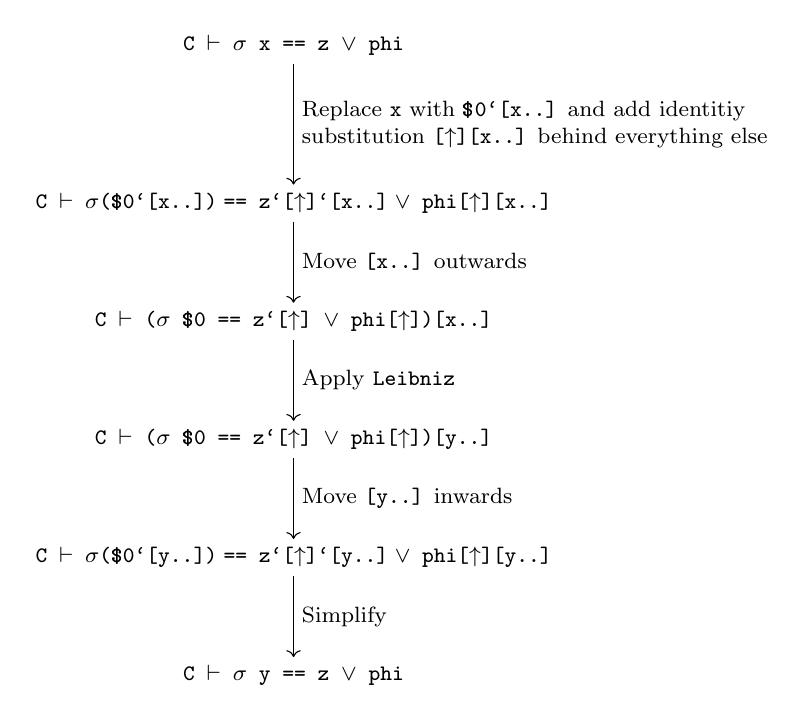
\begin{tikzpicture}\footnotesize
\node (A) at (0,0) {\texttt{C $\vdash$ $\sigma$ x == z $\lor$ phi}};
\node (B) at (0,-2) {\texttt{C $\vdash$ $\sigma$(\$0`[x..])\;== z`[$\uparrow$]`[x..]\;$\lor$ phi[$\uparrow$][x..]}};
\node (C) at (0,-3.5) {\texttt{C $\vdash$ ($\sigma$ \$0 == z`[$\uparrow$] $\lor$ phi[$\uparrow$])[x..]}};
\node (D) at (0,-5) {\texttt{C $\vdash$ ($\sigma$ \$0 == z`[$\uparrow$] $\lor$ phi[$\uparrow$])[y..]}};
\node (E) at (0,-6.5) {\texttt{C $\vdash$ $\sigma$(\$0`[y..])\;== z`[$\uparrow$]`[y..]\;$\lor$ phi[$\uparrow$][y..]}};
\node (F) at (0,-8) {\texttt{C $\vdash$ $\sigma$ y == z $\lor$ phi}};

\path[->] (A) edge node[right,align=left] {\footnotesize Replace \texttt{x} with \texttt{\$0`[x..]} and add identitiy \\\footnotesize substitution \texttt{[$\uparrow$][x..]} behind everything else} (B);
\path[->] (B) edge node[right,align=left] {\footnotesize Move \texttt{[x..]} outwards} (C);
\path[->] (C) edge node[right,align=left] {\footnotesize Apply \texttt{Leibniz}} (D);
\path[->] (D) edge node[right,align=left] {\footnotesize Move \texttt{[y..]} inwards} (E);
\path[->] (E) edge node[right,align=left] {\footnotesize Simplify} (F);
\end{tikzpicture}}

\bigskip\noindent
Sadly this scheme does not work, if the term to rewrite is behind a quantifier, because a substitution \texttt{s} gets turned into \texttt{up s} inside the scope of a quantifier.
To address this, I generalize the idea by using a function \texttt{up\_n} that gives the iterated application of \texttt{up}:

\bigskip
\makebox[\textwidth][c]{
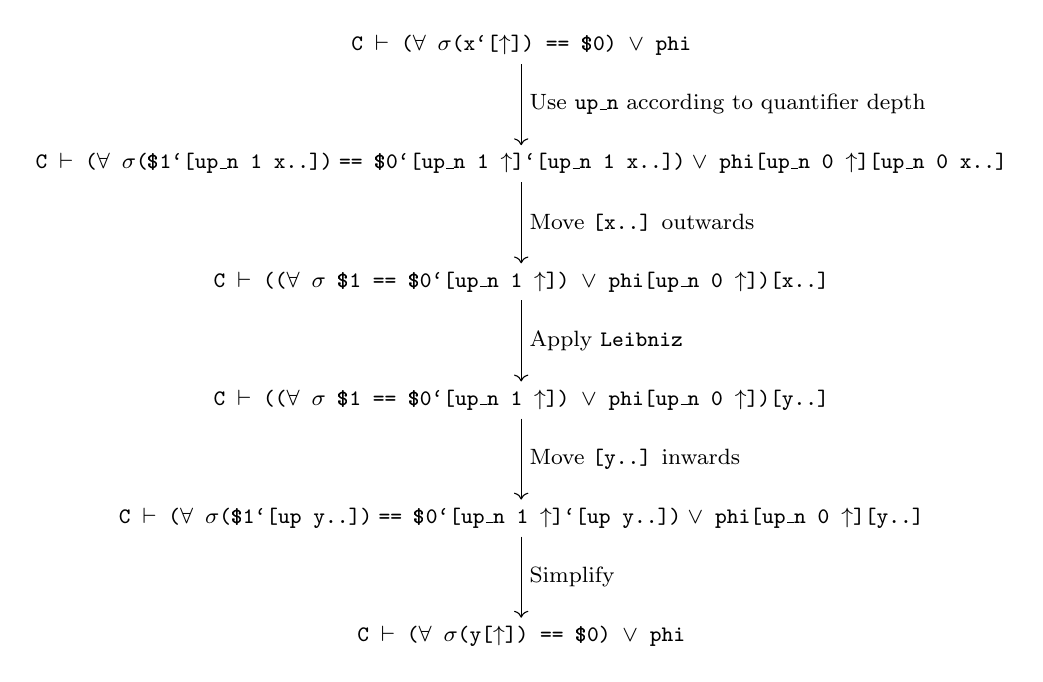
\begin{tikzpicture}\footnotesize
\node (A) at (0,0) {\texttt{C $\vdash$ ($\forall$ $\sigma$(x`[$\uparrow$]) == \$0) $\lor$ phi}};
\node (B) at (0,-1.5) {\texttt{C $\vdash$ ($\forall$ $\sigma$(\$1`[up\_n 1 x..])\;== \$0`[up\_n 1 $\uparrow$]`[up\_n 1 x..])\;$\lor$ phi[up\_n 0 $\uparrow$][up\_n 0 x..]}};
\node (C) at (0,-3) {\texttt{C $\vdash$ (($\forall$ $\sigma$ \$1 == \$0`[up\_n 1 $\uparrow$]) $\lor$ phi[up\_n 0 $\uparrow$])[x..]}};
\node (D) at (0,-4.5) {\texttt{C $\vdash$ (($\forall$ $\sigma$ \$1 == \$0`[up\_n 1 $\uparrow$]) $\lor$ phi[up\_n 0 $\uparrow$])[y..]}};
\node (E) at (0,-6) {\texttt{C $\vdash$ ($\forall$ $\sigma$(\$1`[up y..])\;== \$0`[up\_n 1 $\uparrow$]`[up y..])\;$\lor$ phi[up\_n 0 $\uparrow$][y..]}};
\node (F) at (0,-7.5) {\texttt{C $\vdash$ ($\forall$ $\sigma$(y[$\uparrow$]) == \$0) $\lor$ phi}};

\path[->] (A) edge node[right,align=left] {\footnotesize Use \texttt{up\_n} according to quantifier depth} (B);
\path[->] (B) edge node[right,align=left] {\footnotesize Move \texttt{[x..]} outwards} (C);
\path[->] (C) edge node[right,align=left] {\footnotesize Apply \texttt{Leibniz}} (D);
\path[->] (D) edge node[right,align=left] {\footnotesize Move \texttt{[y..]} inwards} (E);
\path[->] (E) edge node[right,align=left] {\footnotesize Simplify} (F);
\end{tikzpicture}}

\bigskip\noindent
Note that in the case of no quantifiers, we only use \texttt{up\_n 0 s} which is equal to \texttt{s}, so we get essentially the same as in the first example.

\improve{There are some things that could be improved regarding the \texttt{frewrite} tactic:
\begin{itemize}
	\item Support rewriting in hypotheses
	\item Support equivalence rewriting under quantifiers
	\item Support \texttt{frewrite ... at n}
	\item If you want to rewrite under quantifiers, the term needs to be already shifted (in the example above it needs to be \texttt{x`[$\uparrow$]} under the all quantifier). In some cases this is irrelevant because the term is substitution invariant (for example \texttt{num} in PA). Provide a way for the user to register such invariance lemmas and apply them accordingly.
	\item The evar trick from \texttt{fapply} does not work here because I use syntactic matching to find occurrences of the rewrite variable. Thus the user always needs to give the instantiation for variables. But improving this might be tricky...
\end{itemize}}





\end{document}